\documentclass[journal]{IEEEtran}

\usepackage{cite}
\usepackage{amsmath,amssymb}
\usepackage{graphicx}
\usepackage[caption=false,font=footnotesize]{subfig}
\usepackage{booktabs}
\usepackage{tabularx}
\usepackage{array}
\usepackage{multirow}
\usepackage{url}
\usepackage{siunitx}
\usepackage{balance}

\sisetup{detect-all,group-separator={,},group-minimum-digits=4}
\newcommand{\CO}{\mathrm{CO}}
\newcommand{\COtwo}{\mathrm{CO_2}}
\newcommand{\Htwo}{\mathrm{H_2}}
\newcommand{\HtwoO}{\mathrm{H_2O}}
\newcommand{\Otwo}{\mathrm{O_2}}
\newcommand{\CHfour}{\mathrm{CH_4}}
\newcommand{\Ar}{\mathrm{Ar}}
\newcommand{\Ntwo}{\mathrm{N_2}}
\newcommand{\pp}{\,\mathrm{pp}}
\newcommand{\daf}{\mathrm{daf}}

\title{A Reduced-Order, Radially Coupled Model of the BYU Entrained-Flow Coal Gasifier: Formulation, Results, Validation, and Limitations}

\author{Upendra~Singh, Samrudh~Nelli, Arnav~Chauhan, Ashutosh~Ranjan, and Naveen~Saini%
\thanks{ME40249, Introduction to Hydrogen Energy and Utilization. Batch 18. Author identifiers: Upendra Singh (23ME31035), Samrudh Nelli (23ME31025), Arnav Chauhan (23ME10102), Ashutosh Ranjan (23ME3AI34), and Naveen Saini (23MF10027).}}

\markboth{Batch 18 Technical Report}{Reduced-Order Modeling of the BYU Entrained-Flow Gasifier}

\begin{document}
\maketitle

\begin{abstract}
This paper documents the formulation, implementation, numerical checks, and experimental comparison of a reduced-order model for the atmospheric Brigham Young University (BYU) entrained-flow gasifier. The case uses Utah bituminous coal, oxygen-rich primary gas containing argon and steam, and a steam-only secondary stream. Two complementary calculations are used within one modeling workflow: a steady one-dimensional cross-section-averaged plug-flow calculation, and an axisymmetric annular calculation that couples reacting lanes through conservative radial species and enthalpy transport. The chemistry includes competing two-step coal devolatilization, element-balanced volatile allocation, three kinetic-diffusion char reactions, and a four-reaction global gas-phase set. The final radial mesh has 120 annuli and 600 axial stations. At that mesh the tracked C/H/O/N elemental-flow residual is \(2.05\times10^{-6}\%\), the outlet area-average temperature is \(3556.7\) K, and the carbon conversion is \(53.52\%\). The highest recovered temperature reaches the solver's \(4000\) K upper bracket and is therefore not a resolved physical peak. Dry inert-free outlet fractions, normalized over \(\CO\), \(\Htwo\), \(\COtwo\), and \(\CHfour\), are 58.66, 16.68, 24.21, and 0.45 vol\%, respectively; the outlet also retains approximately 4.02 vol\% dry area-average \(\Otwo\) on a total dry-gas basis. The measured BYU outlet values summarized by the reference study are 51.1\% \(\CO\), 24.7\% \(\Htwo\), 23.6\% \(\COtwo\), 0.3\% \(\CHfour\), and 82\% carbon conversion. The radial calculation conserves the tracked elements and exhibits modest changes under grid refinement, but its outlet and profile errors show that numerical consistency is not equivalent to physical validation. The paper makes all spatial, chemical, thermal, and numerical assumptions explicit, maps the study outputs to the required project deliverables, and identifies model upgrades needed before predictive use.
\end{abstract}

\begin{IEEEkeywords}
Coal gasification, entrained-flow reactor, reduced-order model, devolatilization, char conversion, radial mixing, validation, syngas.
\end{IEEEkeywords}

\section{Introduction}
Entrained-flow gasification converts pulverized coal and an oxidant into a hot product gas containing mainly \(\CO\) and \(\Htwo\). In the reactor, particles heat rapidly, release volatile matter, form char, and undergo oxidation and gasification while the gas composition and temperature vary strongly in space. The BYU laboratory reactor is a useful benchmark because its geometry and feed conditions are documented and local gas samples are available for comparison. Brown \emph{et al.} describe measured and predicted local and outlet behavior in this reactor \cite{brown1988}; Mularski and Modlinski later use the BYU case to examine how devolatilization, gas-phase chemistry, and char-conversion modeling affect predictions \cite{mularski2021}.

The present work has two aims. First, it turns the selected BYU case into a transparent executable model whose balances, kinetics, boundary conditions, and numerical choices can be inspected. Second, it evaluates the model against the benchmark quantities that matter for an engineering interpretation: feed description, axial species evolution, radial-axial species and temperature fields, outlet composition and conversion, mesh sensitivity, and comparison with measured profiles.

The model is deliberately described at the level it implements. It is a reduced-order reacting stream-tube model with radial diffusion coupling. It does not solve the Navier--Stokes equations, turbulent momentum transport, Lagrangian particle trajectories, radiative transfer, or a detailed chemical mechanism. The reference calculation in \cite{mularski2021} is a two-dimensional axisymmetric CFD model with substantially more detailed turbulence, particle, radiation, and chemistry closures. Comparisons are consequently interpreted as a model assessment on the same experimental case, not as a claim that the present code reproduces the full reference CFD.

The main contributions and evidence are:
\begin{itemize}
  \item a documented BYU case definition with coal properties, primary and secondary feeds, geometry, and particle-distribution assumptions;
  \item a steady axial reacting calculation and a radially coupled annular calculation with six requested species fields (\(\CO\), \(\Htwo\), \(\COtwo\), \(\HtwoO\), \(\Otwo\), and \(\CHfour\)) and temperature;
  \item explicit chemical and numerical assumptions, including atom-balance closure, the hot-start energy addition, radial mixing closure, and temperature limits;
  \item grid-refinement and particle-size sensitivity results;
  \item centerline and radial comparisons with approximate experimental markers, with measurement and digitization uncertainty disclosed; and
  \item a deliverable-coverage map connecting the technical requirements to report sections, figures, and reproducible project artifacts.
\end{itemize}

\section{Benchmark Problem and Required Output Coverage}
\subsection{Physical system}
The modeled vessel is a straight cylindrical reactor of diameter \(D=0.20\) m and length \(L=1.80\) m, operated at \(101.325\) kPa. The selected coal is Utah bituminous coal. The published case supplies coal and gas rates, proximate and ultimate analyses, and a Rosin--Rammler particle-size distribution \cite{mularski2021}. The two gas inlets are coaxial: the primary stream contains oxygen, argon, and steam and carries the coal; the secondary stream is steam. The input values used by the executable case file are listed in Table~\ref{tab:case}.

\begin{table*}[t]
\caption{BYU case definition used in the simulation. Values marked as assumptions are model inputs rather than measured values tabulated for this case.}
\label{tab:case}
\centering
\small
\begin{tabularx}{\textwidth}{>{\raggedright\arraybackslash}p{0.19\textwidth} X >{\raggedright\arraybackslash}p{0.28\textwidth}}
\toprule
\textbf{Item} & \textbf{Value} & \textbf{Role in model} \\
\midrule
Reactor & \(D=0.20\) m; \(L=1.80\) m; \(P=101325\) Pa & Cylindrical, atmospheric case \cite{mularski2021} \\
Coal & Utah bituminous; \(23.88\) kg/h & Fed with the primary stream \cite{mularski2021} \\
Proximate analysis & Moisture 2.4 wt\%; volatile matter 45.6 wt\%; fixed carbon 43.7 wt\%; ash 8.3 wt\% & As-received basis \cite{mularski2021} \\
Ultimate analysis & C 77.60, H 6.56, N 1.42, S 0.55, O 13.87 wt\% & Dry ash-free basis; O is by difference \cite{mularski2021} \\
Primary stream & \(26.24\) kg/h at \(400\) K; \(85.0\%\ \Otwo\), \(12.6\%\ \Ar\), \(2.4\%\ \HtwoO\) & Coal-bearing oxidant stream \cite{mularski2021} \\
Secondary stream & \(6.62\) kg/h at \(473\) K; pure steam & Coaxial steam stream \cite{mularski2021} \\
Particle size & Rosin--Rammler; range \(1\)--\(85\ \mu\)m; mean \(36\ \mu\)m; spread \(1.033\) & Published distribution \cite{mularski2021} \\
Particle density & \(1300\) kg/m\(^3\) & Provisional engineering assumption used to estimate particle count and surface area \\
Injector dimensions & Primary inner diameter \(13\) mm; secondary outer diameter \(28.6\) mm & Taken from the BYU setup reported by Abani and Ghoniem \cite{abani2013}; not tabulated in \cite{mularski2021} \\
Inlet radial regularization & \(20\%\) uniform-background contribution & Numerical assumption to avoid exactly empty/stagnant annuli \\
Wall and heat transfer & Adiabatic wall; gas and particle share one temperature & Reduced-model assumptions; wall heat loss and separate particle temperature are not solved \\
Hot-start temperature & \(1400\) K at \(z=0\) & Numerical ignition patch; its added energy is quantified in Section~\ref{sec:energy} \\
\bottomrule
\end{tabularx}
\end{table*}

\subsection{Deliverable coverage}
Table~\ref{tab:coverage} gives a direct evidence map for the technical and presentation outputs. The six species fields are shown separately as axial profiles and as radial-axial contours. Results are supported by the saved numerical tables, the source code, the live-demonstration notebook, the class presentation, and this report.
\begin{table*}[t]
\caption{Required output coverage and evidence produced by the project.}
\label{tab:coverage}
\centering
\small
\begin{tabularx}{\textwidth}{>{\raggedright\arraybackslash}p{0.23\textwidth} X X}
\toprule
\textbf{Output} & \textbf{Where addressed in this paper} & \textbf{Reproducible artifact} \\
\midrule
Feed and major gas species & Section~II-A; Table~\ref{tab:case}; outlet composition in Section~VI-B & Case YAML; inlet and outlet CSV files \\
Axial species distribution & Section~VI-A; Fig.~\ref{fig:axial} & Area-average and near-axis profile CSV; plot PNG \\
Species contours & Section~VI-A; Fig.~\ref{fig:species-contours} for \(\CO\), \(\Htwo\), \(\COtwo\), \(\HtwoO\), \(\Otwo\), and \(\CHfour\) & Radial state and contour PNG files \\
Temperature distribution & Section~VI-A; Fig.~\ref{fig:temperature} & Temperature field and area-average temperature CSV/PNG \\
Comparison with the selected journal study and BYU experiment & Sections~VI-B--VI-D; Tables~\ref{tab:outlet-comparison}--\ref{tab:radial-errors} & Digitized marker CSV, comparison figures, and error tables \\
Numerical checks and sensitivity & Sections~V and VI-E; Tables~\ref{tab:grid} and \ref{tab:particle-sweep} & Grid-study and particle-sweep CSV/PNG files \\
Conclusions and limitations & Sections~VIII--IX & This report; source README \\
Report, code, and oral presentation & Source and packaging notes in Section~XI & IEEE PDF and Overleaf source; Batch 18 source package; live-demo notebook; class presentation PDF \\
\bottomrule
\end{tabularx}
\end{table*}

\section{Reference Study and Model Scope}
The selected published study applies an axisymmetric CFD model to the BYU reactor, discretizes the domain with approximately \(10^5\) cells, and reports a grid-independence check. It uses a realizable \(k\)-\(\epsilon\) turbulence model, a discrete-random-walk particle dispersion treatment, discrete-ordinates radiation with a weighted-sum-of-gray-gases model, competing two-step devolatilization rates tuned against FG-DVC, a global gas mechanism checked against detailed chemistry, and empirical kinetic-diffusion char conversion parameters optimized with CBK/E and CBK/G \cite{mularski2021}. The study reports average and maximum local-profile errors for CO, H2, CO2, and H2O; it cautions that H2O values are derived by hydrogen balance and carry about \(\pm14\%\) uncertainty.

The present implementation reuses the same BYU geometry, feed case, published competing two-step devolatilization constants, and optimized char-kinetic parameters. It also uses the published nozzle dimensions from \cite{abani2013} to initialize radial inlet weights. These shared inputs make the cases comparable. The solver architecture and closure set differ substantially: chemistry is solved in axial stream tubes and then operator-split with radial diffusion; there is no solved velocity field, turbulence field, particle trajectory, radiation field, recirculation zone, or interphase momentum coupling. In addition, volatile composition and gas-phase rates are less detailed than in the reference model. The comparison is therefore a transparent reduced-model exercise with known differences in fidelity.

Two spatial formulations are used under the same case definition, not as sequential project phases. The cross-section-averaged plug-flow calculation is a simpler baseline and is used for the particle-size sweep. The radially coupled calculation generates the two-dimensional species and temperature fields and supplies the centerline and radial validation results.

\section{Mathematical Model}
\subsection{State variables and axial species balances}
The axial calculation is steady. For gas species \(i\), \(F_i(z)\) is the molar flow rate in \(\mathrm{mol\,s^{-1}}\). The solid state includes un-devolatilized dry-ash-free coal, \(m_{\rm raw}(z)\), and carbon char, \(m_{\rm char}(z)\), each in \(\mathrm{kg\,s^{-1}}\). The generic axial species balance is
\begin{equation}
\frac{dF_i}{dz}
= A_c\sum_{r=1}^{N_r}\nu_{i,r}\,\dot{\omega}_r
+ S_{i,\mathrm{het}} + S_{i,\mathrm{vol}},
\label{eq:species}
\end{equation}
where \(A_c=\pi D^2/4\), \(\nu_{i,r}\) is the gas-phase stoichiometric coefficient, \(\dot{\omega}_r\) is the global volumetric rate in \(\mathrm{kmol\,m^{-3}\,s^{-1}}\), and the heterogeneous and volatile-release terms are converted to molar flow per unit axial length. Gas composition is computed from the species molar flows. The gas density and superficial velocity follow the ideal-gas relation at the fixed pressure:
\begin{equation}
\rho_g = \frac{P\overline{W}}{R_uT}, \qquad
u_g = \frac{\dot{m}_g}{\rho_g A_c}.
\label{eq:velocity}
\end{equation}
The particles are assigned the gas velocity; slip, particle acceleration, and particle radial motion are not represented.

\subsection{Energy balance and temperature recovery}
Rather than integrate temperature as an independent state, the code recovers temperature at each axial state from a total enthalpy-flow constraint:
\begin{equation}
H(T,\mathbf{F},m_{\rm char},m_{\rm raw},m_{\rm ash})=H_0.
\label{eq:enthalpy}
\end{equation}
Species enthalpies include standard formation enthalpy and sensible enthalpy, with constant species heat capacities. Solid char, ash, and raw coal use constant heat-capacity approximations. A bracketed scalar root solve over \(280\)--\(4000\) K finds \(T\); if the target is outside that enthalpy range, the state is returned at the nearer bracket endpoint. The reference state is set by the \(1400\) K hot-start patch, not by the cold feed enthalpy alone. Because reaction products carry their formation enthalpies, the constant-total-enthalpy closure converts reaction progress into sensible temperature without separately integrating a heat-release source.

This is an adiabatic closure. The wall boundary condition and radiative exchange are not solved. The single-temperature assumption sets particle temperature \(T_p\) equal to gas temperature \(T_g\), although real coal particles can depart from gas temperature during rapid heating. Coal moisture is added immediately as vapor at the inlet; there is no separate liquid-droplet evaporation model. The clipping behavior means that a reported \(4000\) K point indicates the numerical upper bracket, not a validated prediction of a physical flame temperature.

The BYU case does not provide a calorific value in the selected input table. The code estimates the dry-ash-free higher heating value (HHV) from the ultimate analysis with the Channiwala--Parikh correlation \cite{channiwala2002}:
\begin{equation}
\begin{split}
\mathrm{HHV}_{\daf}\;[\mathrm{MJ\,kg^{-1}}]
=0.3516C+1.16225H-0.1109O\\
\quad+0.0628N+0.10465S,
\end{split}
\label{eq:hhv}
\end{equation}
where \(C,H,O,N,S\) are the dry-ash-free mass percentages. The resulting coal formation enthalpy is then estimated from the complete-combustion products and this HHV. This introduces a fuel-energy estimate rather than a measured calorific value.

\subsection{Coal devolatilization and volatile allocation}
Coal devolatilization uses the competing two-step model (C2SM). For the remaining raw coal, the two rates are
\begin{equation}
k_j(T_p)=A_j\exp\left(-\frac{E_j}{R_uT_p}\right),\quad j\in\{1,2\},
\label{eq:arrhenius}
\end{equation}
\begin{align}
\dot{m}_{\rm vol} &= \left(\alpha_1k_1+\alpha_2k_2\right)m_{\rm raw},\\
\dot{m}_{\rm char} &= \left[(1-\alpha_1)k_1+(1-\alpha_2)k_2\right]m_{\rm raw}.
\end{align}
The implementation uses \(A_1=4.269\times10^4\,\mathrm{s^{-1}}\), \(E_1=3.71\times10^7\,\mathrm{J\,kmol^{-1}}\), \(\alpha_1=0.246\), \(A_2=9.785\times10^6\,\mathrm{s^{-1}}\), \(E_2=8.993\times10^7\,\mathrm{J\,kmol^{-1}}\), and \(\alpha_2=0.931\), transcribed from Table 5 of \cite{mularski2021}. The activation energies are converted to \(\mathrm{J\,mol^{-1}}\) in the code before evaluating \eqref{eq:arrhenius}.

The mass released as volatiles does not determine a unique gas composition. Three elemental equations (C, H, O) cannot determine five product amounts (\(\CO\), \(\COtwo\), \(\Htwo\), \(\HtwoO\), and \(\CHfour\)) without additional closure assumptions. The implementation therefore states two explicit allocation choices: all available volatile oxygen is first assigned to CO (\(f_{\mathrm{O}\rightarrow\mathrm{CO}}=1\)); half the hydrogen remaining after water formation is allocated to methane (\(f_{\mathrm{H}\rightarrow\mathrm{CH_4}}=0.5\)), with the rest assigned to hydrogen. Product allocations are clipped by the available C, H, and O inventories in a fixed sequence so they cannot exceed the elemental inventory.

Char is treated as pure carbon. Nitrogen is represented as \(\Ntwo\). Any volatile carbon left after CO, CO2, and methane allocation is retained as a soot/char surrogate and is subsequently consumed by the same char reaction set. This keeps the tracked C/H/O/N balances closed, but is not equivalent to the reference study's explicit tar species and tar chemistry. Sulfur is not represented by a gas species or included in the tracked elemental-balance diagnostic; hence the reported balance check is specifically for C, H, O, and N, not for all elements in the fuel.

\subsection{Heterogeneous char conversion}
Three surface reactions are included:
\begin{align}
\mathrm{C(s)}+\tfrac12\Otwo &\rightarrow \CO, \label{eq:charox}\\
\mathrm{C(s)}+\COtwo &\rightarrow 2\CO, \label{eq:boud}\\
\mathrm{C(s)}+\HtwoO &\rightarrow \CO+\Htwo. \label{eq:steam}
\end{align}
They represent partial oxidation, Boudouard gasification, and steam gasification. Their relative heat effects are important: \eqref{eq:charox} releases heat, whereas \eqref{eq:boud} and \eqref{eq:steam} consume heat. For each reaction, a kinetic coefficient and an external-diffusion coefficient are combined as resistances in series:
\begin{equation}
k_{\mathrm{eff},r}=\left(\frac{1}{k_{s,r}}+\frac{1}{k_d}\right)^{-1}, \qquad
\dot{m}_{C,r}=k_{\mathrm{eff},r}A_p p_{\mathrm{ox},r}.
\label{eq:char_rate}
\end{equation}
The diffusion closure is \(k_d=C_{\mathrm{diff}}[(T_g+T_p)/2]^{0.75}/d_p\), with \(C_{\mathrm{diff}}=5.0\times10^{-12}\). The surface coefficient is
\begin{equation}
k_{s,r}=A_rT_p^{\beta_r}\exp\left(-\frac{E_r}{R_uT_p}\right).
\end{equation}
The optimized BYU parameter set in Table~\ref{tab:char-kinetics} is taken from Table 6 of \cite{mularski2021}. Those values are fitted for the reference coal and case; they should not be interpreted as universal coal constants. Particle external surface area is based on a fixed particle diameter and estimated particle count. Shrinking particle area, internal pore diffusion, ash effects, and evolving pore structure are omitted.

\begin{table*}[t]
\caption{Optimized char kinetic parameters used in the code. \(E\) is shown after conversion from \(\mathrm{J\,kmol^{-1}}\) to \(\mathrm{J\,mol^{-1}}\).}
\label{tab:char-kinetics}
\centering
\small
\begin{tabular}{lrrrr}
\toprule
Reaction & \(A\) & \(E\) (J/mol) & \(\beta\) & Oxidizer\\
\midrule
\(\mathrm{C+0.5O_2\rightarrow CO}\) & \(1.298{\times}10^{-3}\) & \(1.324{\times}10^5\) & 1.233 & \(\Otwo\)\\
\(\mathrm{C+CO_2\rightarrow2CO}\) & \(6.60{\times}10^{-2}\) & \(1.385{\times}10^5\) & -0.263 & \(\COtwo\)\\
\(\mathrm{C+H_2O\rightarrow CO+H_2}\) & \(1.877{\times}10^{-3}\) & \(1.588{\times}10^5\) & -0.124 & \(\HtwoO\)\\
\bottomrule
\end{tabular}
\end{table*}

\subsection{Global gas-phase chemistry}
The model has four gas-phase global reactions:
\begin{align}
\CO+\tfrac12\Otwo &\rightarrow \COtwo, \\
\Htwo+\tfrac12\Otwo &\rightarrow \HtwoO, \\
\CO+\HtwoO &\rightleftharpoons \COtwo+\Htwo, \\
\CHfour+\HtwoO &\rightarrow \CO+3\Htwo.
\end{align}
Each forward rate has Arrhenius dependence multiplied by species concentrations raised to the orders in Table~\ref{tab:gas-kinetics}. The reversible water-gas-shift (WGS) rate is multiplied by \(1-Q/K_p\), with \(Q=[\COtwo][\Htwo]/([\CO][\HtwoO])\) and \(K_p=\exp(4577.8/T-4.33)\). This compact mechanism omits intermediate hydrocarbon, tar, radical, and nitrogen chemistry; it has no turbulence-chemistry interaction closure.

\begin{table*}[t]
\caption{Global gas-phase rate set as implemented. Values are code inputs; their complete source-to-parameter provenance is not established in the project files. They are not asserted to be the full mechanism or parameter set of \cite{mularski2021}. Concentrations are evaluated in \(\mathrm{kmol\,m^{-3}}\).}
\label{tab:gas-kinetics}
\centering
\small
\begin{tabularx}{\textwidth}{>{\raggedright\arraybackslash}p{0.27\textwidth} >{\raggedright\arraybackslash}p{0.25\textwidth} c c X}
\toprule
\textbf{Reaction} & \textbf{Rate orders} & \(\boldsymbol{A}\) & \(\boldsymbol{E}\) (J/mol) & \textbf{Heat of reaction used in enthalpy bookkeeping} \\
\midrule
\(\CO+0.5\Otwo\rightarrow\COtwo\) & \([\CO]^1[\Otwo]^{0.25}[\HtwoO]^{0.5}\) & \(2.239\times10^{12}\) & \(1.70\times10^5\) & \(-282.99\) kJ/mol CO \\
\(\Htwo+0.5\Otwo\rightarrow\HtwoO\) & \([\Htwo]^1[\Otwo]^{0.5}\) & \(1.00\times10^{14}\) & \(1.70\times10^5\) & \(-241.83\) kJ/mol H2 \\
\(\CO+\HtwoO\rightleftharpoons\COtwo+\Htwo\) & \([\CO]^1[\HtwoO]^1\) & \(2.75\times10^9\) & \(8.40\times10^4\) & \(-41.20\) kJ/mol forward reaction \\
\(\CHfour+\HtwoO\rightarrow\CO+3\Htwo\) & \([\CHfour]^1[\HtwoO]^1\) & \(3.00\times10^8\) & \(1.26\times10^5\) & \(+206.00\) kJ/mol CH4 \\
\bottomrule
\end{tabularx}
\end{table*}

The exact gas-phase constants and rate orders deserve particular caution. The code records these values but marks their provenance for verification. Consequently, the paper reports their implemented values for reproducibility and does not claim that the whole set has been independently validated against the selected reference mechanism. This uncertainty is relevant to the outlet residual oxygen and composition errors.

\subsection{Radially coupled annular calculation}
The radial calculation divides the vessel cross-section into \(N_r\) concentric annuli and the length into \(N_z\) axial stations. Each annulus carries a local vector of gas molar flows, char flow, raw-coal flow, and enthalpy flow. The inlet weights are constructed from the primary core and secondary annulus nozzle dimensions with a uniform-background fraction of 0.20; the discrete weights are normalized so integrated inlet stream rates match the case rates. This regularization avoids empty annuli, but it is not a measured radial velocity or species profile.

At each axial step, the local chemistry increment from the uncoupled reacting lane is applied to the previously mixed state. A backward-Euler finite-volume solve then diffuses each gas species between neighboring annuli. The same internal-face flux is entered with opposite signs in the adjacent control volumes, making the discrete radial species exchange conservative. Species enthalpy is carried with the diffusing molar flux, followed by an implicit radial heat-conduction step. The centerline has the axisymmetric symmetry condition; the wall has zero radial species and heat flux in the implemented closure.

The turbulent diffusivity is estimated from
\begin{equation}
D_t = \min(C_m U_b R,\ 0.20~\mathrm{m^2\,s^{-1}}), \quad C_m=0.05,
\end{equation}
where \(U_b\) is the area-weighted bulk velocity and \(R=D/2\). Species and heat diffusivities use \(D_t/Sc_t+D_m\) and \(D_t/Pr_t+D_m\), respectively, with \(Sc_t=0.70\), \(Pr_t=0.90\), \(D_m=10^{-5}\,\mathrm{m^2\,s^{-1}}\), and the same \(0.20\,\mathrm{m^2\,s^{-1}}\) cap. The coefficient \(C_m\), background inlet fraction, Schmidt number, Prandtl number, and cap form a reduced closure, not values inferred from experimental turbulence measurements.

Operator splitting is a computational choice. Chemistry increments are generated from independently solved axial lanes, then applied to a radially exchanged state at the next station. If the mixed state cannot supply a consumed trace species, the reaction increment is scaled to keep species nonnegative. This ensures robust local bookkeeping but means local chemistry does not continuously feed back into the same axial increment. No radial momentum equation updates local velocity in response to radial mass exchange.

\section{Numerical Method and Verification}
\subsection{Integration and grid}
The cross-section-averaged axial calculation integrates the species and solid states with LSODA, a stiff-capable variable-step integrator, using relative tolerance \(10^{-6}\), absolute tolerance \(10^{-12}\), and maximum step \(L/200\). Temperature recovery uses a bracketed Brent root solve. The radial grid uses \(N_r=120\) annuli and \(N_z=600\) axial stations for the reported final calculation. The axial spacing is \(L/(N_z-1)\), and annular areas use exact differences of circular face areas. Radial species and thermal transport are solved with tridiagonal backward-Euler systems.

\subsection{Balance diagnostic}
At the final mesh, the maximum absolute tracked-element-flow discrepancy is \(2.0549\times10^{-6}\%\). The diagnostic accounts for gas species, solid char, and residual raw coal and checks C, H, O, and N from inlet to outlet. This very small numerical residual is evidence that the implemented allocation and transport steps conserve these tracked elements. It is not evidence that the chosen kinetic parameters or closures represent the real reactor, nor does it include sulfur.

\subsection{Grid refinement}
Table~\ref{tab:grid} compares four meshes. Dry-gas fractions in this table use total dry gas as denominator, including argon, nitrogen, and residual oxygen; this is distinct from the inert-free reporting basis used later. Refinement from \(80\times400\) to \(120\times600\) changes area-average outlet temperature by \(9.08\) K, carbon conversion by \(-1.28\) percentage points, and the listed total-dry CO, H2, and CO2 fractions by \(-0.65\), \(-0.74\), and \(+0.80\) percentage points.

\begin{table*}[t]
\caption{Mesh sensitivity of the radial calculation. Species values are outlet dry vol\% on a total dry-gas basis, including inerts and residual oxygen. Peak temperature is the recovered field maximum and is capped at the solver's upper bracket.}
\label{tab:grid}
\centering
\small
\begin{tabular}{rrrrrrrr}
\toprule
\(N_r\) & \(N_z\) & \(T_{\mathrm{out,area}}\) (K) & \(X_C\) (\%) & CO (\%) & H2 (\%) & CO2 (\%) & Max. C/H/O/N residual (\%)\\
\midrule
20 & 100 & 3447.9 & 62.47 & 55.95 & 17.25 & 14.62 & \(4.69\times10^{-7}\)\\
40 & 200 & 3530.3 & 57.41 & 53.46 & 14.87 & 18.73 & \(6.28\times10^{-7}\)\\
80 & 400 & 3547.6 & 54.80 & 50.71 & 14.98 & 19.86 & \(1.19\times10^{-6}\)\\
120 & 600 & 3556.7 & 53.52 & 50.07 & 14.24 & 20.66 & \(2.05\times10^{-6}\)\\
\bottomrule
\end{tabular}
\end{table*}

The trend suggests decreasing changes in outlet temperature at the two finest meshes, but carbon conversion and species continue to shift. This four-mesh sequence is a practical resolution check, not a formal order-of-accuracy study. It does not test the radial mixing closure, the operator-splitting error, the chemistry, or the temperature-ceiling issue. No conclusion about physical accuracy follows from mesh stability alone.

\section{Results}
\subsection{Axial development and spatial fields}
Fig.~\ref{fig:axial} shows area-average axial species and temperature behavior. The profiles summarize the radial states and should not be interpreted as centerline curves. The radial model also predicts strong radial variation because the primary and secondary feeds enter different coaxial regions and mix downstream.

\begin{figure*}[t]
\centering
\subfloat[Area-average species profiles]{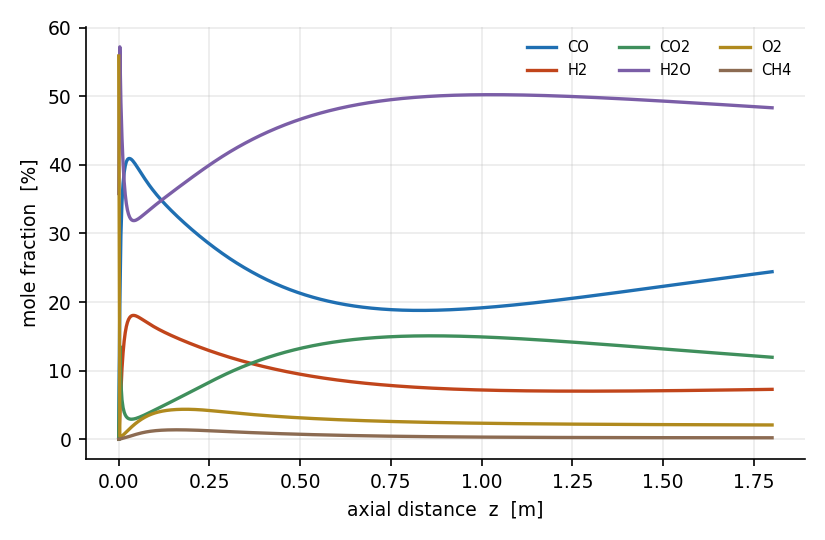
\includegraphics[width=0.48\textwidth]{figures/fig_area_average_species.png}\label{fig:axial-species}}
\hfill
\subfloat[Area-average temperature profile]{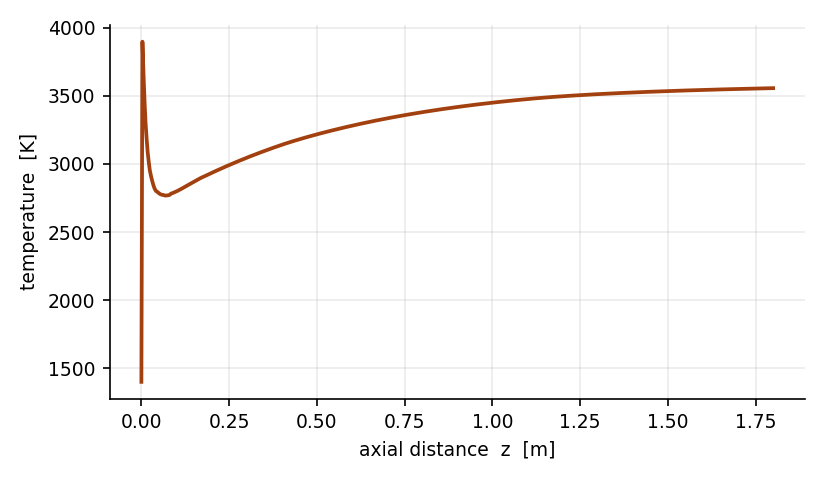
\includegraphics[width=0.48\textwidth]{figures/fig_area_average_temperature.png}\label{fig:axial-temp}}
\caption{Area-weighted axial averages from the radially coupled calculation. The hot start and temperature upper-bracket behavior are described in Sections~VI-A and VII.}
\label{fig:axial}
\end{figure*}

\begin{figure*}[t]
\centering
\subfloat[\(\CO\)]{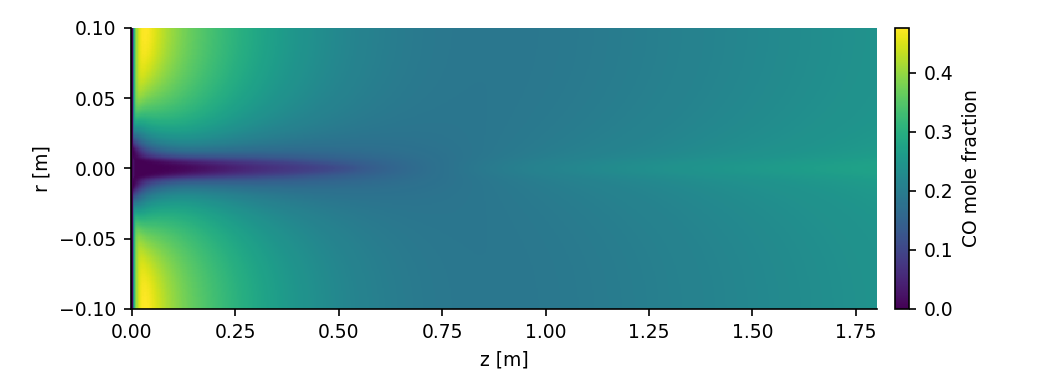
\includegraphics[width=0.48\textwidth]{figures/fig_contour_CO.png}}\hfill
\subfloat[\(\Htwo\)]{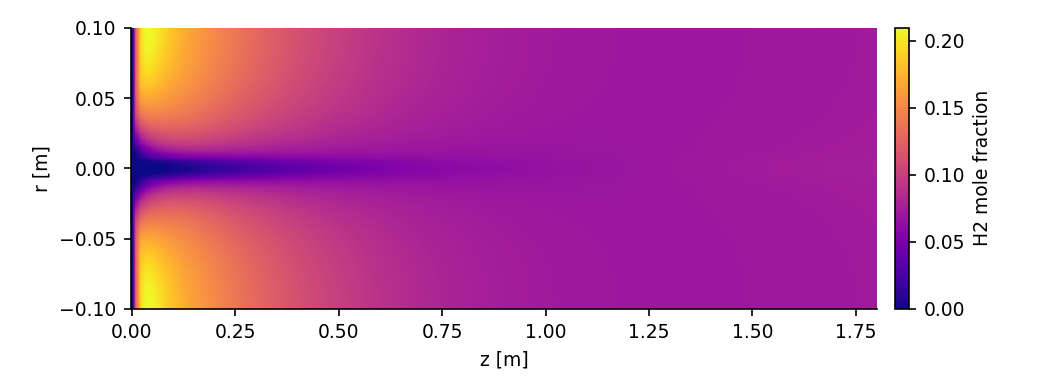
\includegraphics[width=0.48\textwidth]{figures/fig_contour_H2.png}}\\
\subfloat[\(\COtwo\)]{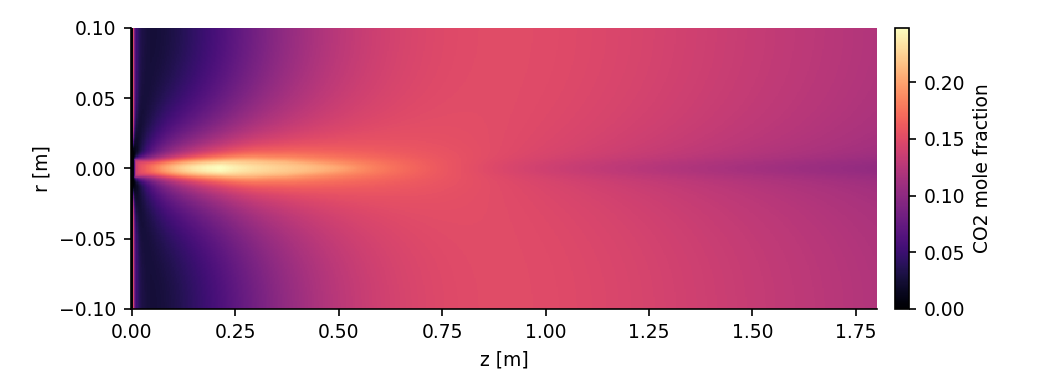
\includegraphics[width=0.48\textwidth]{figures/fig_contour_CO2.png}}\hfill
\subfloat[\(\HtwoO\)]{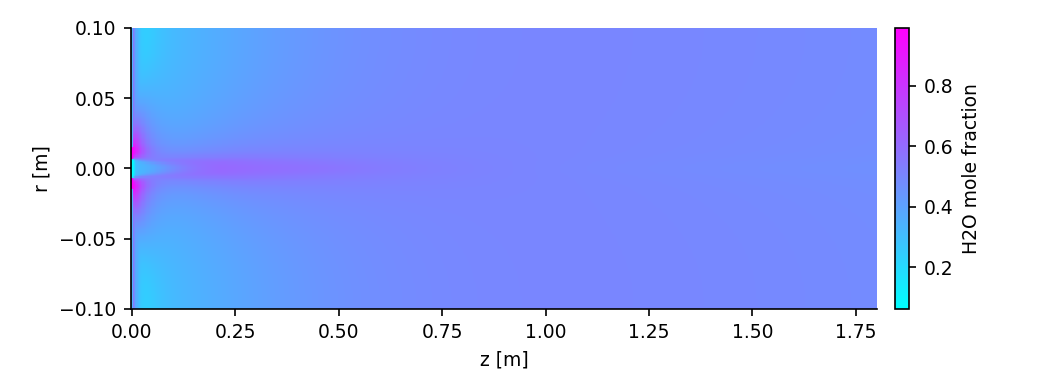
\includegraphics[width=0.48\textwidth]{figures/fig_contour_H2O.png}}\\
\subfloat[\(\Otwo\)]{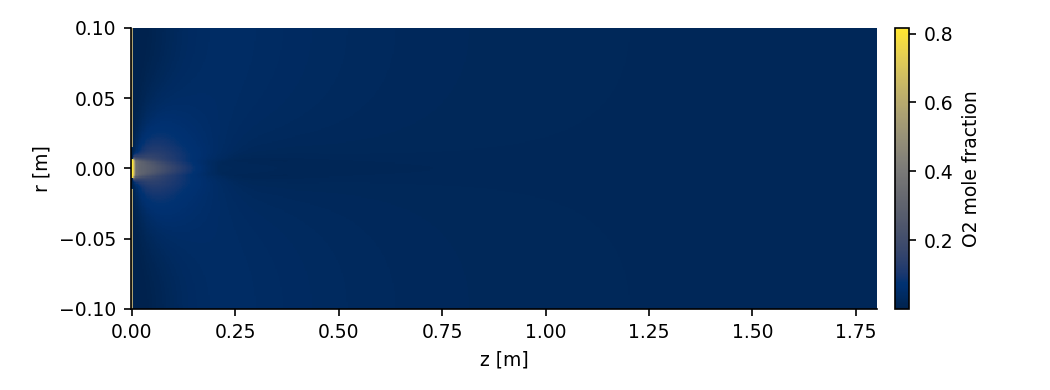
\includegraphics[width=0.48\textwidth]{figures/fig_contour_O2.png}}\hfill
\subfloat[\(\CHfour\)]{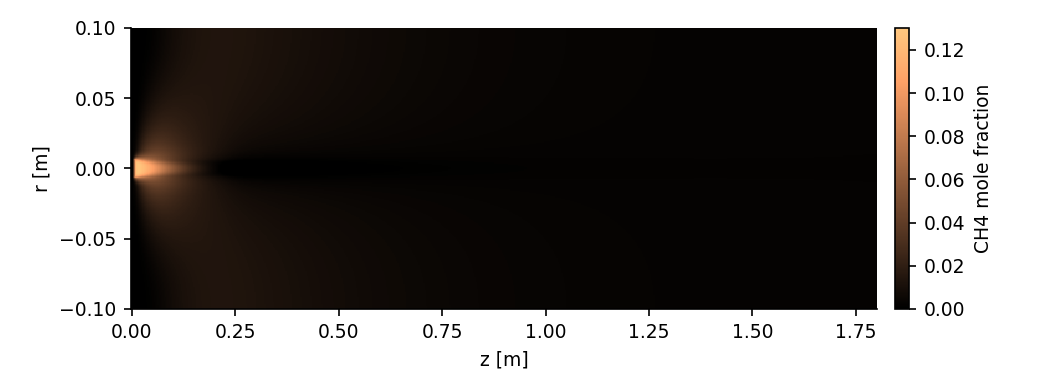
\includegraphics[width=0.48\textwidth]{figures/fig_contour_CH4.png}}
\caption{Computed radial-axial mole-fraction fields. These are model fields from the reduced annular calculation, not experimental contour measurements.}
\label{fig:species-contours}
\end{figure*}

\begin{figure*}[t]
\centering
\subfloat[Temperature field]{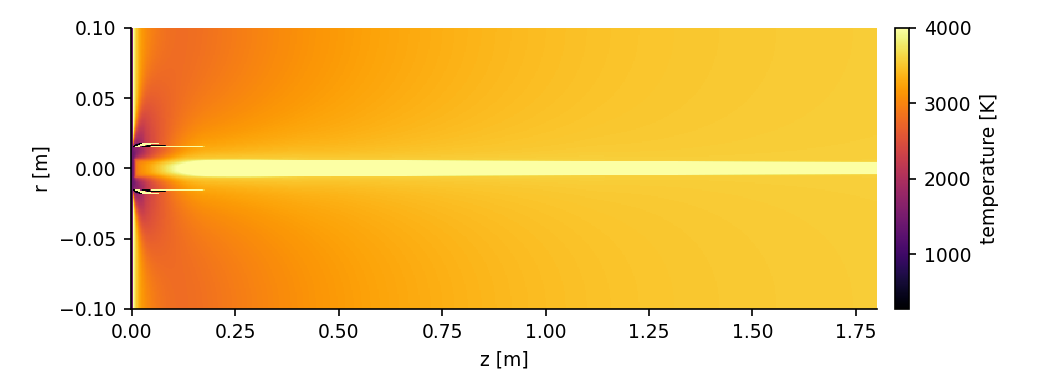
\includegraphics[width=0.57\textwidth]{figures/fig_contour_T.png}\label{fig:temp-contour}}
\hfill
\subfloat[Area-average axial temperature]{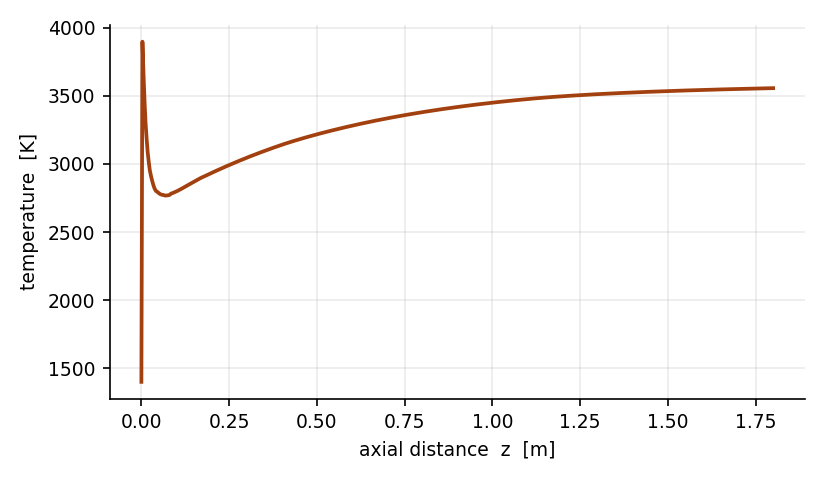
\includegraphics[width=0.38\textwidth]{figures/fig_area_average_temperature.png}\label{fig:temp-line}}
\caption{Temperature distribution from the model. A recovered value of \(4000\) K is the upper enthalpy-root bracket; the reported maximum is clipped and is not treated as a measured or converged peak temperature.}
\label{fig:temperature}
\end{figure*}

Across the cross-section, the area-average outlet values from the saved radial profile are \(T=3556.7\) K, \(\CO=24.42\%\), \(\Htwo=7.27\%\), \(\COtwo=11.95\%\), \(\CHfour=0.210\%\), \(\HtwoO=48.33\%\), \(\Otwo=2.079\%\), \(\Ar=5.195\%\), and \(\Ntwo=0.537\%\) on the model's wet mole-fraction basis. The area-average outlet gas still contains oxygen. On a total dry-gas basis, area-average \(\Otwo\) is about \(4.02\%\), indicating that oxygen is not fully consumed in the calculation. At least three components could contribute: the assumed radial inlet distribution and mixing, the simplified gas reaction set, and the absence of solved turbulent flow and recirculation. The present data do not isolate these causes.

\subsection{Outlet composition and conversion comparison}
For comparison with the dry-gas benchmark, the model's four dry, inert-free product species are renormalized to sum to 100\%, excluding steam, argon, nitrogen, and residual oxygen. This is a reporting normalization and does not mean that oxygen is physically absent from the outlet. Table~\ref{tab:outlet-comparison} contrasts the model with the measured BYU values summarized in the selected study. The clearest discrepancies are 7.56 percentage points excess CO, 8.02 points deficient H2, and 28.48 points lower carbon conversion. CO2 is within 0.61 points under this outlet normalization, but pointwise validation in Section~VI-C shows that the axial and radial shapes still differ.

For product species \(i\in\{\CO,\Htwo,\COtwo,\CHfour\}\), the reporting basis is
\begin{equation}
x_{i,\mathrm{dry,inert\!-\!free}}
=100\frac{F_{i,\mathrm{out}}}{\sum_{j\in\{\CO,\Htwo,\COtwo,\CHfour\}}F_{j,\mathrm{out}}}.
\end{equation}
Carbon conversion is calculated from carbon remaining in the outlet char and raw coal:
\begin{equation}
X_C=1-\frac{m_{\mathrm{char,out}}+y_Cm_{\mathrm{raw,out}}}
{y_Cm_{\mathrm{DAF,in}}},
\end{equation}
where \(y_C\) is the coal's dry-ash-free carbon mass fraction. This metric counts all unconverted char, including the surplus-carbon surrogate formed during volatile allocation.

\begin{table}[t]
\caption{Dry inert-free outlet comparison. The model fractions are normalized over CO, H2, CO2, and CH4 only.}
\label{tab:outlet-comparison}
\centering
\footnotesize
\begin{tabular}{lrrr}
\toprule
Quantity & Model & BYU data & Difference\\
\midrule
CO (vol\%) & 58.66 & 51.1 & \(+7.56\) pp\\
H2 (vol\%) & 16.68 & 24.7 & \(-8.02\) pp\\
CO2 (vol\%) & 24.21 & 23.6 & \(+0.61\) pp\\
CH4 (vol\%) & 0.45 & 0.3 & \(+0.15\) pp\\
Carbon conversion (\%) & 53.52 & 82 & \(-28.48\) pp\\
\bottomrule
\end{tabular}
\end{table}

The cold-gas-efficiency diagnostic is \(25.95\%\), calculated as
\begin{equation}
\mathrm{CGE}=\frac{\sum_{i\in\{\Htwo,\CO,\CHfour\}}F_{i,\mathrm{out}}\mathrm{LHV}_i}
{m_{\mathrm{DAF,in}}\mathrm{HHV}_{\daf}}.
\end{equation}
Its numerator uses lower heating values of 10.8, 12.6, and 35.8 MJ/Nm\(^3\) for H2, CO, and CH4, respectively, with a reference molar volume of \(22.4\) L/mol; the fuel denominator is based on the dry-ash-free coal HHV estimated by \eqref{eq:hhv}. It is reported as a code-defined diagnostic, not as an independently validated plant efficiency. Because the current chemistry leaves residual oxygen and substantially underpredicts conversion, this CGE should be read with those limitations in view.

\subsection{Centerline profile comparison}
The axial validation compares the innermost radial-cell center at \(r=0.00083\) m with approximate centerline experimental markers digitized from Fig. 9 of \cite{mularski2021}. Marker coordinates are not raw tabulated measurements: the project digitization has estimated uncertainties of approximately \(\pm0.3\) mole-fraction percentage point and \(\pm0.01\) m in axial position. The error definition is the mean or maximum absolute composition difference in percentage points at the digitized axial samples:
\begin{equation}
e_{\mathrm{abs},i} = |x_{i,\mathrm{model}}-x_{i,\mathrm{exp}}|\times100.
\end{equation}
Table~\ref{tab:axial-errors} compares the calculated errors with the error values reported by the paper for its own CFD model. The latter are a contextual benchmark and not a re-analysis of our model using the paper's original simulation fields.

\begin{table*}[t]
\caption{Near-axis centerline error comparison. Errors are absolute mole-fraction differences in percentage points. The selected study's reported values refer to its own model.}
\label{tab:axial-errors}
\centering
\small
\begin{tabular}{lrrrrrr}
\toprule
Species & \(n\) & Present mean (pp) & Present max (pp) & Reference mean (pp) & Reference max (pp) & Scored?\\
\midrule
CO & 7 & 12.811 & 25.722 & 4.82 & 18.48 & Yes\\
H2 & 6 & 10.498 & 13.027 & 5.47 & 7.95 & Yes\\
CO2 & 7 & 7.268 & 14.458 & 4.72 & 10.15 & Yes\\
H2O & 6 & 25.541 & 31.337 & 9.58 & 20.22 & No; derived and uncertain\\
\bottomrule
\end{tabular}
\end{table*}

\begin{figure*}[t]
\centering
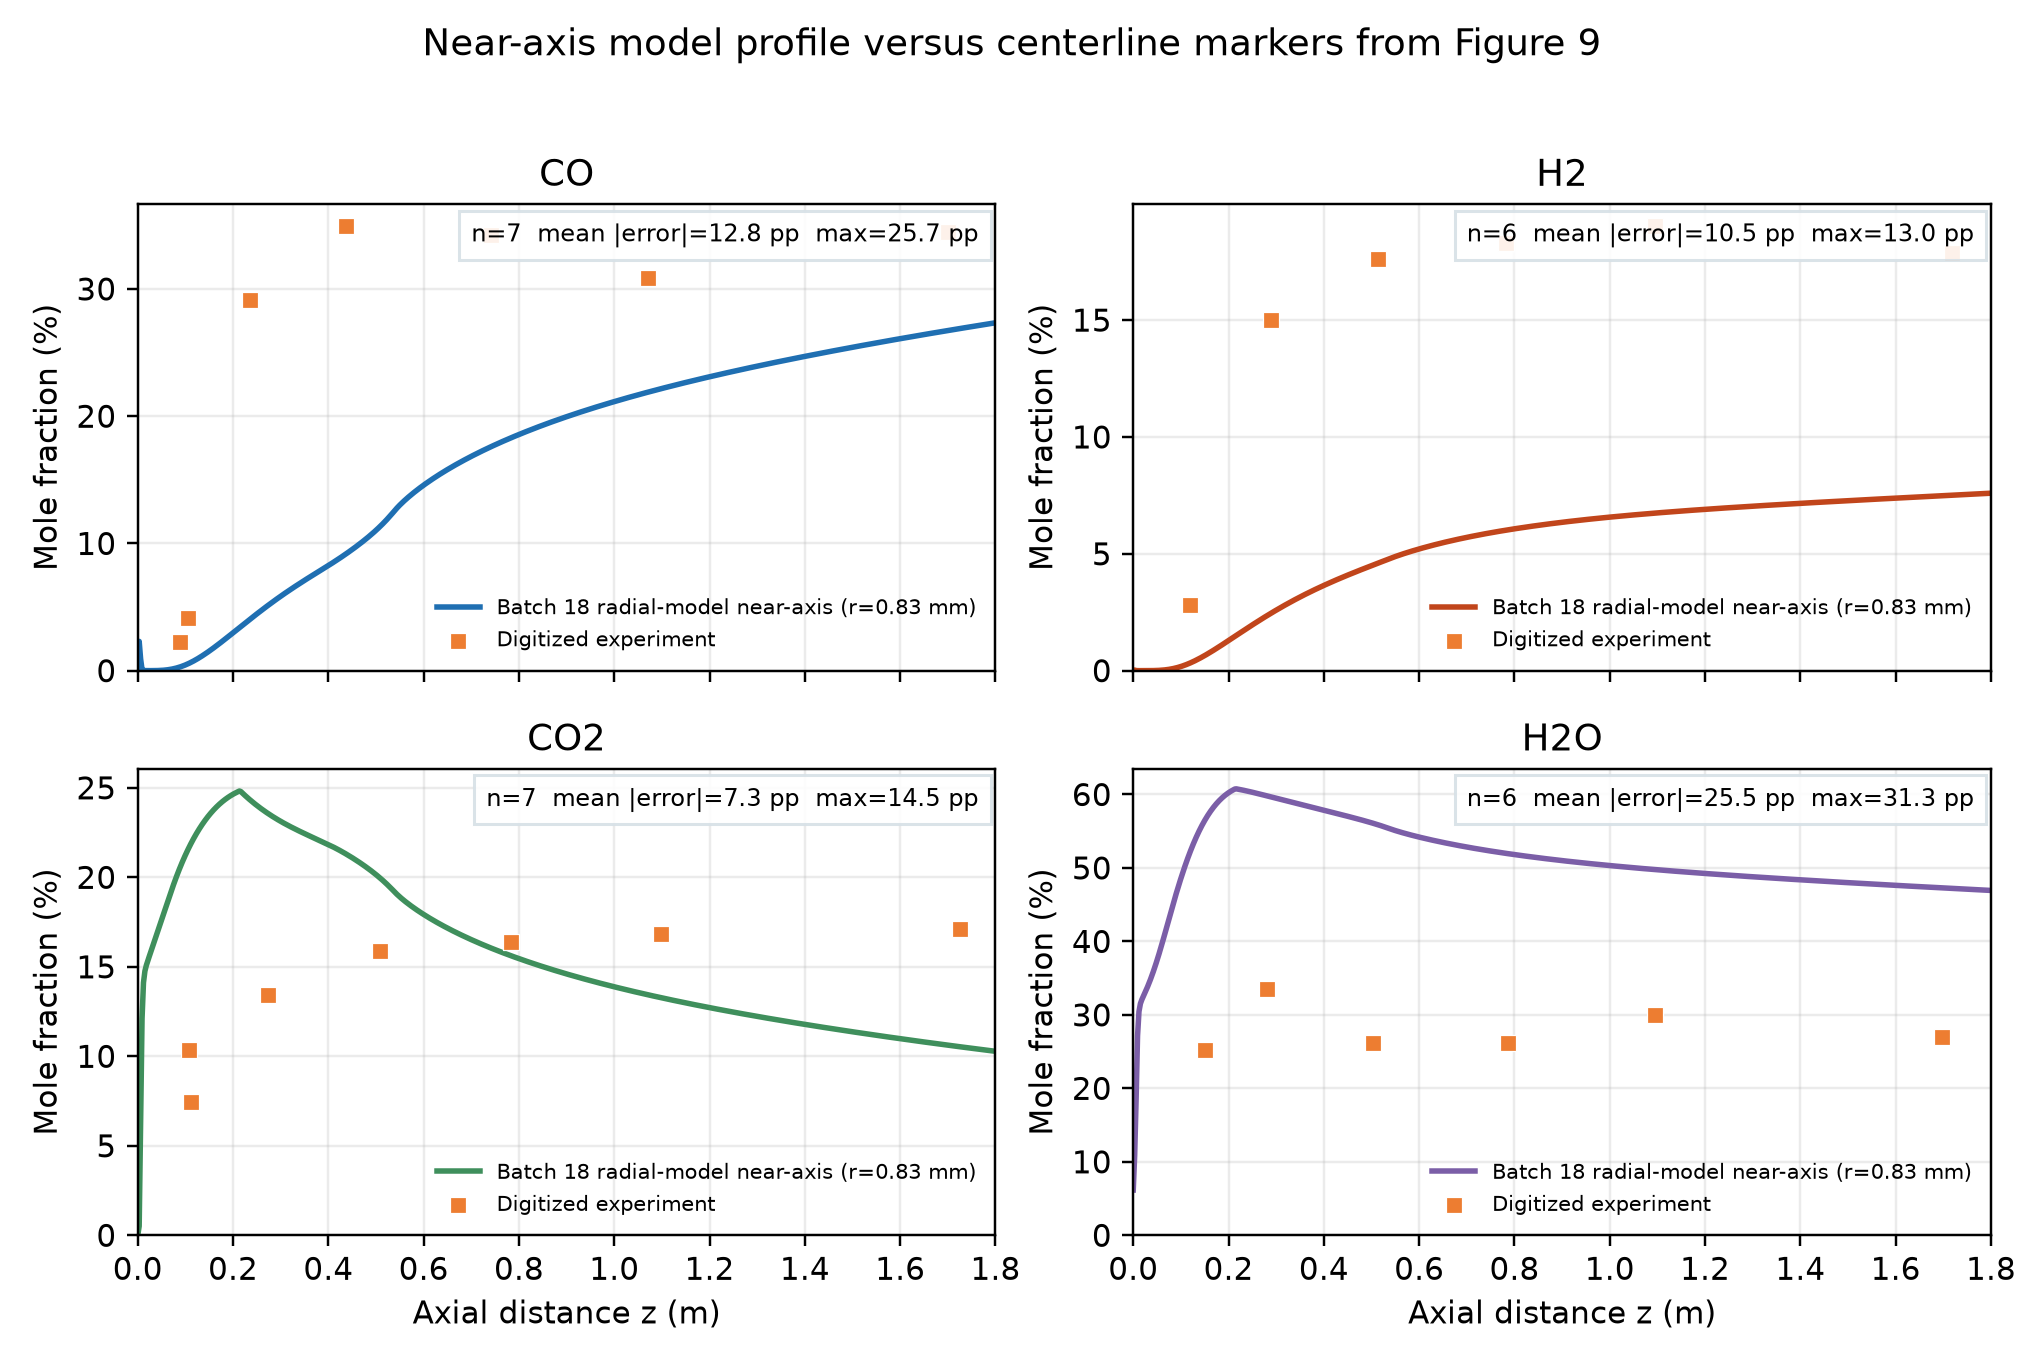
\includegraphics[width=0.90\textwidth]{figures/fig_validation_axial_centerline.png}
\caption{Near-axis axial model profiles and digitized centerline markers. The reported H2O marker series is shown for context but not scored because the source study derives H2O by elemental balance and assigns it approximately \(\pm14\%\) uncertainty.}
\label{fig:validation-axial}
\end{figure*}

The centerline errors for the three scored species exceed the reference model's reported mean and maximum errors. Therefore, the current radial model does not reproduce the measured axial profiles at the reference-model level of agreement. The differences are consistent with the simplified flow, mixing, particle, thermal, and gas-chemistry closures, but the current analysis cannot attribute an error fraction to any one closure.

\subsection{Radial profile comparison}
Radial measurements at eight axial stations (\(z=0.13,0.20,0.28,0.34,0.51,0.81,1.12,\) and \(1.73\) m) are digitized from Figs. 12--14 of \cite{mularski2021}. The source plot's orange experimental markers are retained. Their approximate digitization uncertainty is \(\pm0.001\) m in radius and \(\pm0.5\) percentage point in mole fraction. Pooled mean and maximum absolute errors are shown in Table~\ref{tab:radial-errors}; H2O is excluded for the same balance-derived-data reason as in the axial comparison.

\begin{table}[t]
\caption{Pooled radial-profile validation error over all scored stations.}
\label{tab:radial-errors}
\centering
\footnotesize
\begin{tabular}{lrrr}
\toprule
Species & \(n\) & Mean absolute error (pp) & Maximum (pp)\\
\midrule
CO & 34 & 8.541 & 24.223\\
H2 & 36 & 7.023 & 15.327\\
CO2 & 35 & 6.737 & 20.507\\
\bottomrule
\end{tabular}
\end{table}

\begin{figure*}[t]
\centering
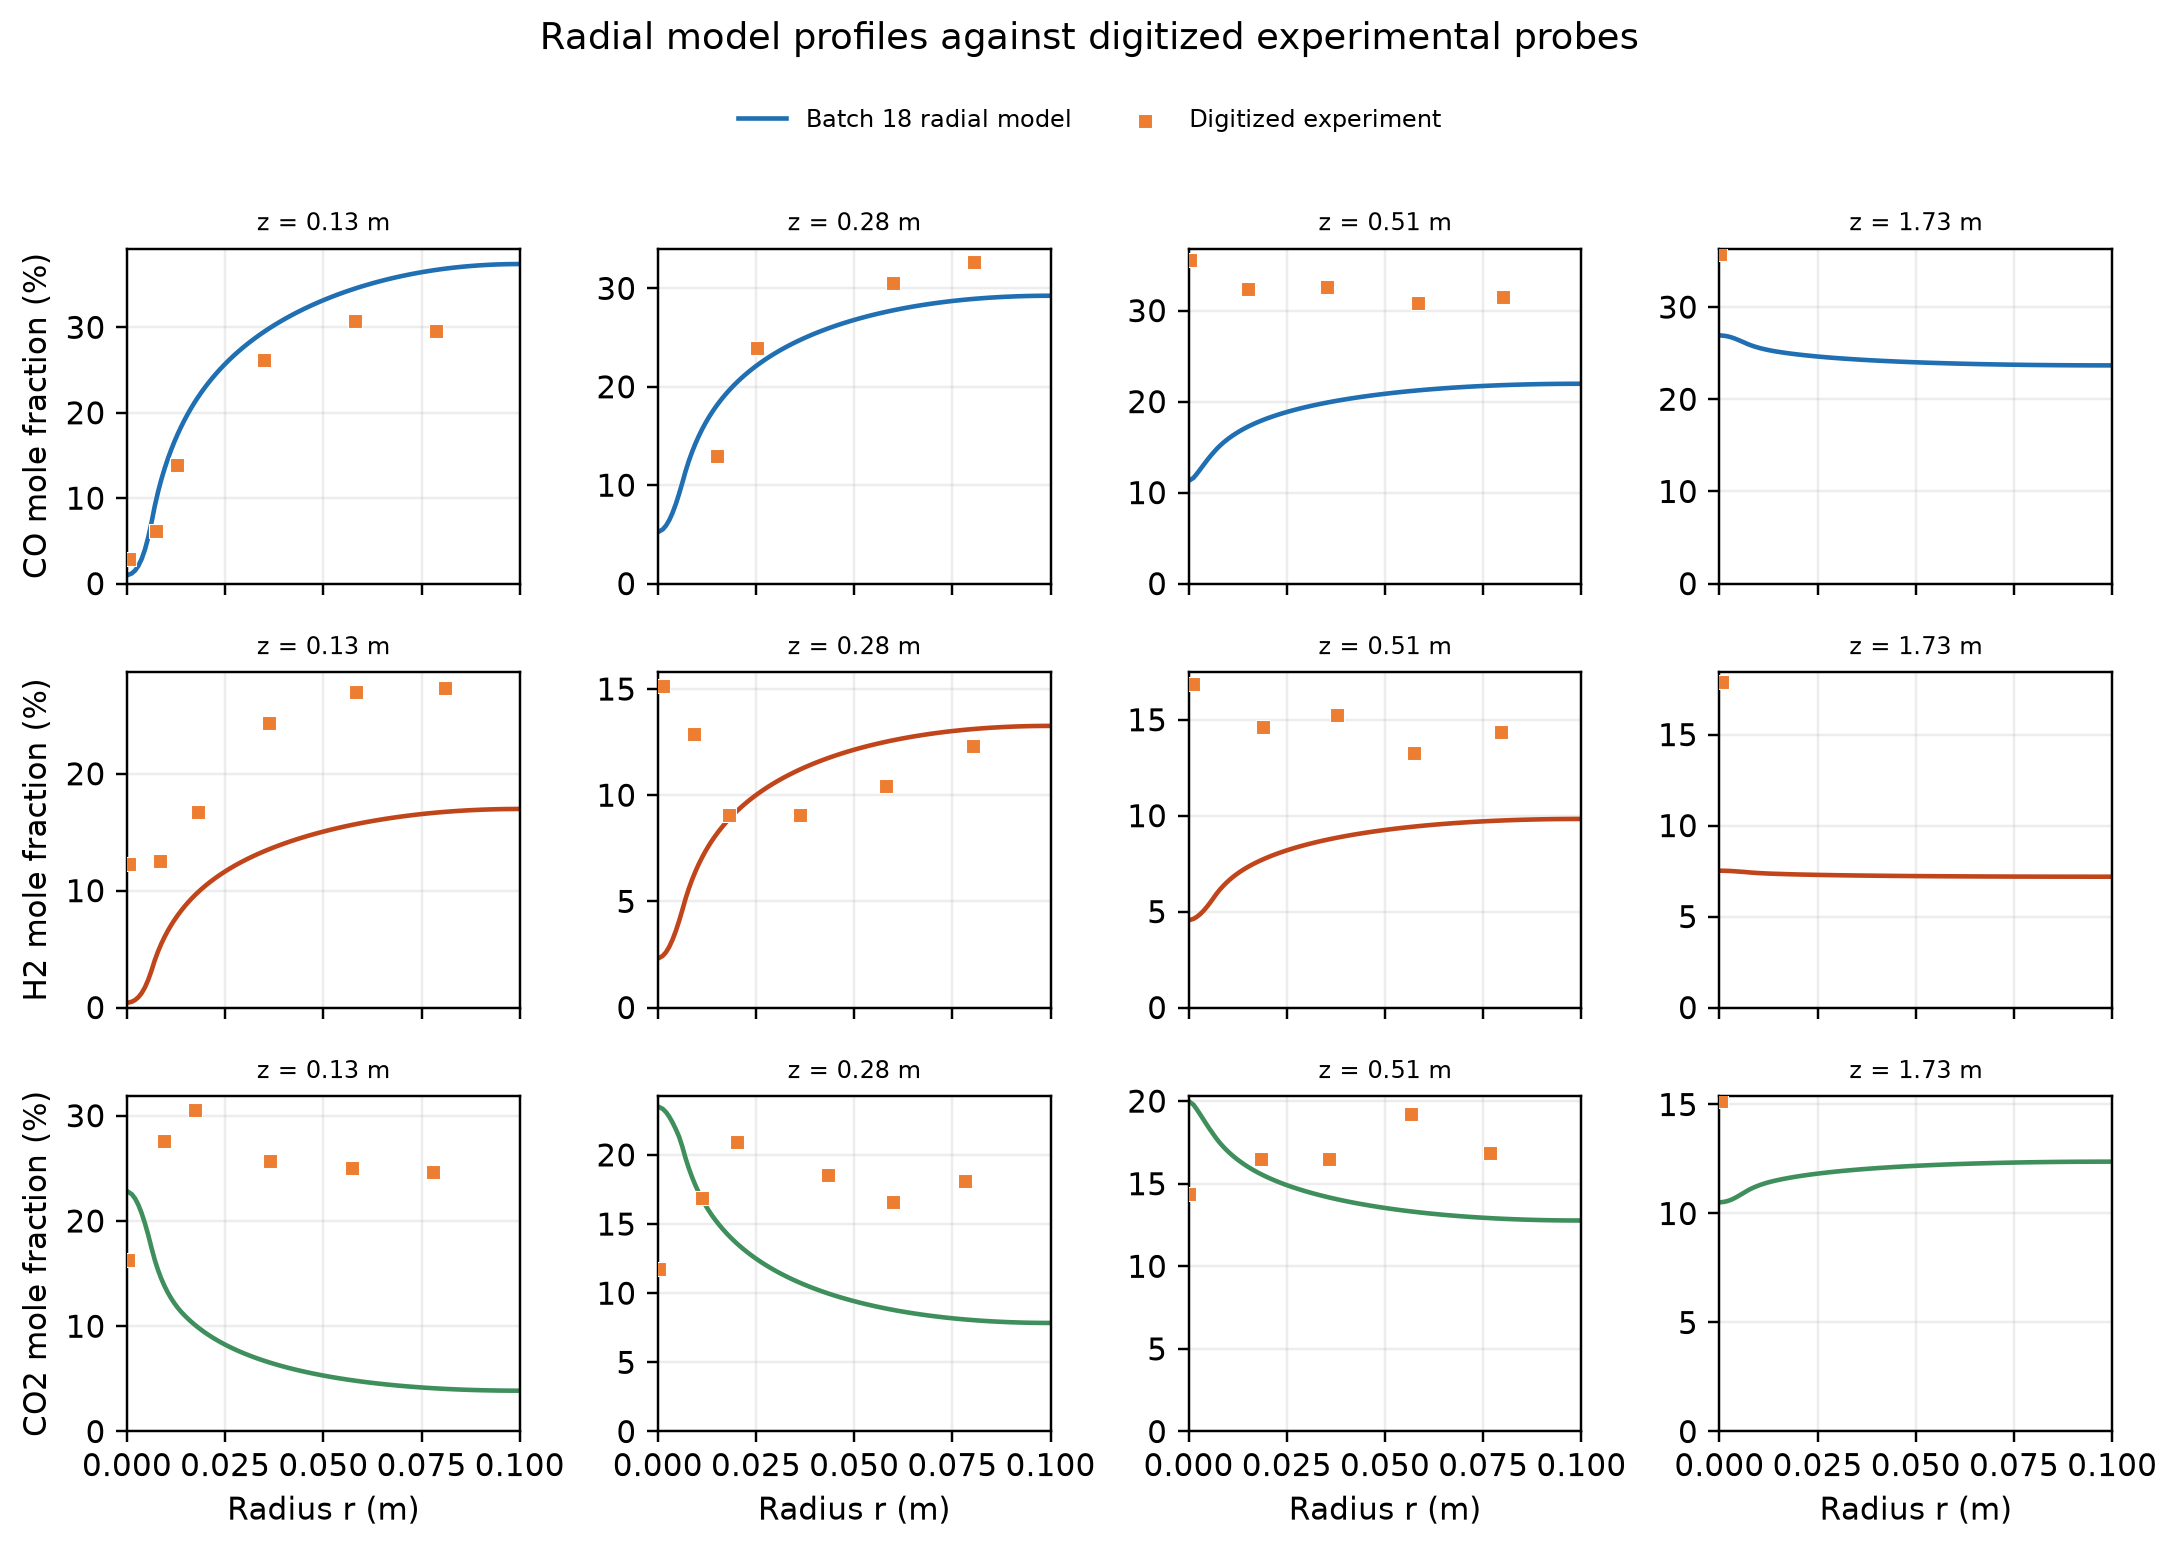
\includegraphics[width=0.94\textwidth]{figures/fig_validation_radial_profiles.png}
\caption{Radial concentration profiles at representative axial stations, compared with digitized experimental markers. The complete error calculation includes all eight measurement stations, even though the plot displays a subset.}
\label{fig:validation-radial}
\end{figure*}

The radial pooled means are smaller than some of the centerline errors, but maximum local differences remain as high as 24.22 percentage points for CO and 20.51 points for CO2. A pooled average can hide strong local disagreements, so these values do not justify a general claim of agreement. Digitization uncertainty is also not a substitute for the original raw measurement uncertainty.

\subsection{Particle-size sensitivity}
The independent particle-size sweep uses the cross-section-averaged axial calculation. It varies Rosin--Rammler scale diameter over 20, 36, and 60 \(\mu\)m and spread parameter over 0.7, 1.033, and 1.5, with six mass-weighted size bins; a 36-\(\mu\)m monodisperse case is included. All cases return approximately 100\% carbon conversion, \(71.65\%\) cold-gas efficiency, and nearly identical composition. Table~\ref{tab:particle-sweep} summarizes representative results.

\begin{table}[t]
\caption{Representative particle-size-sweep outputs from the cross-section-averaged calculation.}
\label{tab:particle-sweep}
\centering
\footnotesize
\begin{tabular}{lrrrr}
\toprule
Distribution & Scale (\(\mu\)m) & \(X_C\) (\%) & CGE (\%) & H2/CO\\
\midrule
Rosin--Rammler & 20 & 100.00 & 71.65 & 0.451\\
Rosin--Rammler & 36 & 100.00 & 71.65 & 0.451\\
Rosin--Rammler & 60 & 100.00 & 71.65 & 0.451\\
Monodisperse & 36 & 100.00 & 71.65 & 0.451\\
\bottomrule
\end{tabular}
\end{table}

\begin{figure}[t]
\centering
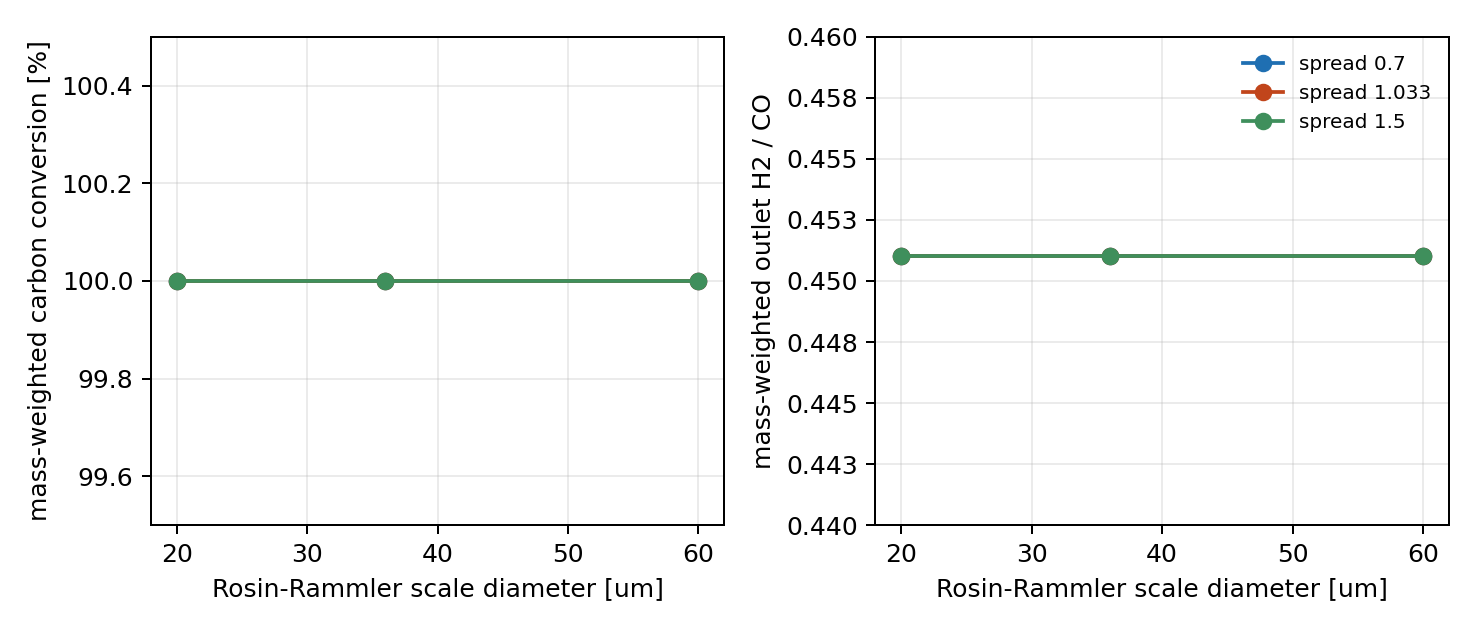
\includegraphics[width=\columnwidth]{figures/fig_particle_size_sensitivity.png}
\caption{Particle-size sweep. The flat result diagnoses complete-burnout saturation in this axial calculation; it does not demonstrate that particle size has no physical effect.}
\label{fig:particle-sweep}
\end{figure}

The sweep is inconclusive for particle-size influence because conversion has saturated at 100\%. The reference study reports 83\% carbon conversion for a 36-\(\mu\)m monodisperse case and 77\% for the full 1--85-\(\mu\)m distribution, versus 82\% measured \cite{mularski2021}. Those values are reported here only as outcomes of the reference study; they are not predictions reproduced by this reduced model. A useful follow-on study would lower the excessive burnout tendency or extend the sensitivity to particle density, char kinetics, and residence time and then verify that a physically meaningful unsaturated regime is obtained.

\section{Energy Initialization and Interpretation}
\label{sec:energy}
The \(1400\) K hot-start is applied to avoid a cold, non-igniting plug-flow solution. A one-dimensional reacting stream without recirculation or radiation feedback has no mechanism to establish a flame from the cold inlet streams at the outset. In the implementation, the hot-start raises the enthalpy reference for the mixture before axial integration. Its equivalent added energy is approximately \(19.35\) kW, about \(9.75\%\) of coal HHV input. This is an artificial energy input used to initiate chemistry; it is not generated by the coal and is not a solved burner heat-transfer process.

This patch affects temperature-dependent devolatilization and reaction rates from the beginning of the calculation. It can therefore alter the subsequent thermal and chemical solution, not merely shift the temperature plot. A predictive version should replace it with a physical ignition/burner boundary condition or a resolved recirculation/radiation model. The current temperature field also reaches the \(4000\) K enthalpy-root bracket. Since the bracket itself sets this ceiling, no physical interpretation should be assigned to the clipped peak.

\section{Discussion}
\subsection{What the model establishes}
The source code produces two complementary spatial calculations within one reproducible workflow. The cross-section-averaged plug-flow result supports the simpler axial baseline and particle-size sweep; the radially coupled result supplies the contours and the centerline and radial profile comparisons. Its strongest verified numerical property is conservation of C/H/O/N within the implemented state and transport formulation. Grid refinement has a modest final-step effect on outlet area-average temperature, but composition and carbon conversion remain more sensitive than the temperature alone.

\subsection{What the model does not establish}
The \(2.05\times10^{-6}\%\) tracked-element residual establishes arithmetic consistency for C/H/O/N, not physical correctness. The final outlet comparison shows a 28.48-point conversion deficit and an 8.02-point H2 deficit. The model also leaves approximately 4.02 vol\% dry area-average oxygen and reaches a temperature ceiling. Axial and radial errors show local mismatches. Together, these observations prevent a claim that the model is a validated predictor of reactor performance.

Several limitations may contribute, but their individual effects have not been isolated:
\begin{itemize}
  \item no momentum equation, turbulence closure, recirculation, or residence-time distribution;
  \item assumed coaxial inlet weights and radial turbulent diffusivity rather than solved jet mixing;
  \item no particle trajectories, particle slip, particle radial dispersion, shrinking diameter, or separate particle temperature;
  \item no radiative heat transfer or wall heat loss, and a \(1400\) K hot-start energy addition;
  \item simplified volatile allocation without explicit tar and a sulfur-free product set;
  \item a four-reaction gas mechanism whose exact parameter provenance is incomplete in the project record; and
  \item numerical clipping at the 4000 K enthalpy bracket and a mixing/chemistry operator split.
\end{itemize}

\subsection{Why a reduced implementation was used}
A reduced formulation allows the full chain from feed analysis to species and energy balances, chemistry, radial transport, numerical integration, and validation to remain inspectable and demonstrable. The same reduction creates the limitations above. Reproducing the reference CFD would require a gas-flow solver, turbulence model, Lagrangian particles and dispersion, radiation, tar-aware devolatilization, validated gas chemistry, and coupled heterogeneous surface chemistry. These components are coupled and require consistent boundary conditions, model parameters, and numerical methods. The present implementation does not claim to substitute for that solver. It uses common benchmark inputs and published char/devolatilization parameter subsets to study and expose how a transparent reduced closure behaves.

\section{Conclusions}
This work documented and evaluated a reduced-order BYU entrained-flow gasifier model. The model uses the published geometry, coal, stream conditions, competing two-step devolatilization parameters, and optimized char-kinetic parameters, while a conservative finite-volume radial-diffusion closure extends reacting axial lanes across the reactor radius. The model supplies feed tables, axial species profiles, radial-axial species and temperature fields, grid and particle-size studies, and comparisons with digitized axial and radial experimental data.

At \(120\times600\), the reported outlet area-average temperature is \(3556.7\) K and carbon conversion is \(53.52\%\). Dry inert-free CO/H2/CO2/CH4 are 58.66/16.68/24.21/0.45 vol\%, compared with 51.1/24.7/23.6/0.3 vol\% summarized for the BYU measurements. Carbon conversion is 28.48 percentage points below the reported 82\% experiment. The dry outlet still contains about 4.02 vol\% area-average O2, and the local maximum temperature is limited by the 4000 K root bracket. Centerline mean absolute errors for CO/H2/CO2 are 12.81/10.50/7.27 points; pooled radial mean errors are 8.54/7.02/6.74 points. H2O comparison is shown only as context because the experimental value is derived and carries large uncertainty.

The mesh study shows small changes in the finest-grid outlet temperature but does not eliminate sensitivity in conversion and composition or establish accuracy. The particle-size sweep is inconclusive because the axial calculation burns out all cases. The correct engineering conclusion is therefore that the project achieved a transparent, balance-checked reduced solver and a complete comparison workflow, while the current model does not reproduce all measurements and needs physical and chemical improvements before predictive use.

\section{Recommended Model Improvements}
The following changes follow directly from the diagnosed issues:
\begin{enumerate}
  \item verify and document every gas-phase pre-exponential factor, activation energy, rate order, concentration unit, and reverse-rate convention against a primary source; then rerun the outlet and profile comparisons;
  \item remove the artificial hot-start by implementing a physical burner or recirculation boundary condition and account for wall radiation and heat losses;
  \item solve gas-phase momentum and turbulence, including recirculation and a consistent chemistry--turbulence interaction closure;
  \item transport particles with separate particle temperature, slip, size-dependent trajectories, dispersion, shrinking surface area, and residence time;
  \item replace the ad hoc volatile split and surplus-carbon-to-char approximation with an explicit tar-aware devolatilization and cracking model;
  \item include sulfur-bearing products or explicitly expand the case's tracked element set; and
  \item conduct mesh, axial-step, radial-mixing-parameter, hot-start, particle-density, and kinetic-parameter sensitivity studies with unsaturated conversion and un-clipped temperature outcomes.
\end{enumerate}
These are model-development recommendations, not results already achieved in the present simulations.

\section{Reproducibility and Project Artifacts}
\subsection{Reproduction}
The project source tree contains the case definition in \texttt{case/byu\_case.yaml}, model modules in \texttt{src/gasifier/}, run scripts in \texttt{scripts/}, validation data and provenance in \texttt{data/validation/}, and computed tables and plots in \texttt{report/}. The conda environment file and notebook kernel instructions accompany the live-demo notebook. The saved radial-profile table and headline metrics are under \texttt{report/}; grid and particle-size results are in \texttt{report/grid\_independence.csv} and \texttt{report/particle\_size\_sensitivity.csv}. The validation errors are in \texttt{report/validation\_errors.csv} and \texttt{report/validation\_radial\_errors.csv}.

The Overleaf package consists of this \LaTeX{} source, \texttt{references.bib}, a \texttt{figures/} directory, and \texttt{README.md}. Upload the source ZIP as a new Overleaf project and set \texttt{Batch18\_IEEE\_Report.tex} as the main document. The local build uses the IEEEtran journal class and BibTeX.

\subsection{Complete output set}
The deliverables associated with the study are:
\begin{itemize}
  \item the technical report as a compiled IEEE-style PDF and an editable Overleaf source package;
  \item the Python source code, BYU case input, saved numerical CSV outputs, plots, and validation-marker data;
  \item the live-demo Jupyter notebook, which explains the governing ideas and demonstrates an educational solver step by step;
  \item the class presentation PDF; and
  \item the traceable analysis evidence listed in Table~\ref{tab:coverage}.
\end{itemize}
The live-demo notebook is a pedagogical demonstration and is not the numerical source of the 120-by-600 results reported in this paper. The result numbers here refer to the saved project radial calculation and associated CSV files.

\section*{Acknowledgment}
The authors thank the experimental researchers whose published BYU measurements and model descriptions made a reproducible benchmark comparison possible.

\balance
\bibliographystyle{IEEEtran}
\bibliography{references}
\end{document}
